\documentclass{beamer}

\usepackage{../Research}

\newcommand{\F}{\mathcal F}
\newcommand{\curly}[1]{\left\{ #1 \right\}}
\newcommand{\paren}[1]{\left( #1 \right)}
\newcommand{\defn}{\underline}

\title{VC-density in model theoretic structures}
\author{Anton Bobkov}
\date{June 3, 2015}


\begin{document}

\maketitle

\begin{frame}
	Suppose we have an (infinite) collection of sets $\F$. \\
	We define the \defn{shatter function} $\pi_\F \colon \N \arr \N$ of $\F$

	\begin{align*}
		\pi_\F(n) = \max \{ &\text {\# of atoms in the boolean algebra generated by $\mathcal S$} \\
		            &\mid \mathcal S \subset \F \text{ with } |\mathcal S| = n\}
	\end{align*}
\end{frame}

\begin{frame}
	Example: Let $\F$ consist of all half-planes in the plane.
	\begin{figure}[p]
    \centering
    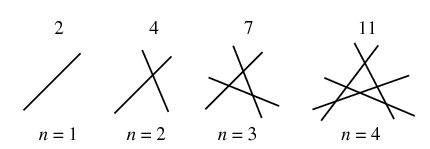
\includegraphics[scale=0.75]{lines.png}
	\end{figure}
	\begin{align*}
		\pi_\F(1) = 2 \ \ \  \pi_\F(2) = 4 \ \ \  \pi_\F(3) = 7  \ \ \ \pi_\F(4) = 11
	\end{align*}
	\begin{align*}
		\pi_\F(n) = n^2/2 + n/2 + 1
	\end{align*}
\end{frame}

\begin{frame}
More examples: \\
	\begin{enumerate}
		%\item Half-planes in the plane: $\pi_\F(n) = n^2/2 + n/2 + 1$
		\item Disks in the plane:	$\pi_\F(n) = n^2 - n + 2$
		\item Balls in $\R^3$: $\pi_\F(n) = n^3/3 - n^2 + 8n/3$
		\item Intervals in the line: $\pi_\F(n) = 2n$
		\item Finite subsets of $\N$: $\pi_\F(n) = 2^n$
		\item Convex polygons in the plane: $\pi_\F(n) = 2^n$
	\end{enumerate}
\end{frame}

\begin{frame}
	\begin{Theorem} [Sauer-Shelah '72]
		The shatter function is either $2^n$ or bounded by a polynomial.
	\end{Theorem}
	\begin{Definition}
		Suppose the growth of the shatter function of $\F$ is polynomial.
		Let $\vc(\F)$ be the infimum of all positive reals $r$ such that
		\begin{align*}
			\pi_\F(n) = O(n^r)
		\end{align*}
		Call $\vc(\F)$ the \defn{vc-density} of $\F$.
		If the shatter function grows exponentially, we let $\vc(\F) := \infty$.
	\end{Definition}
\end{frame}

\begin{frame}
	\frametitle{Applications}
	\begin{itemize}
		\item Model Theory (NIP theories)
		\item VC-Theorem in probability (Vapnik-Chervonenkis '71)
		\item Computational learning theory (PAC learning, Warmuth conjecture)
		\item Computational geometry
		\item Functional analysis (Bourgain-Fremlin-Talagrand theory)
		\item Abstract topological dynamics (tame dynamical systems)
	\end{itemize}
\end{frame}

\begin{frame}
	\frametitle{History}
	\begin{itemize}
		\item VC-dimension defined by Vapnik-Chervonenkis '71
		\item NIP theories studied by Shelah '71
		\item vc-density in model theoretic context introduced by Aschenbrenner, Dolich, Haskell, Macpherson, Starchenko '13
	\end{itemize}
\end{frame}

\begin{frame}
	\frametitle{Model Theory}
	Model Theory studies definable sets in first-order structures.
	\begin{align*}
		(\Q, 0, 1, +, \cdot, \leq)
	\end{align*}
	\begin{align*}
		\phi(x) := \paren{\exists y \ y \cdot y = x}
	\end{align*}
	$\phi(\Q)$ defines the set of rationals that are a square.
\end{frame}

\begin{frame}
	\begin{align*}
		(\R, 0, 1, +, \cdot, \leq)
	\end{align*}
	\begin{align*}
		\phi(x) := \paren{\exists y \ y \cdot y = x}
	\end{align*}
	$\phi(\R)$ defines the set $[0, \infty)$.
\end{frame}

\begin{frame}
	\begin{align*}
		(\R, 0, 1, +, \cdot, \leq)
	\end{align*}
	\begin{align*}
		\psi(x_1, x_2) := (x_1 \cdot x_1 + x_2 \cdot x_2 \leq 1.5) \wedge (x_1\cdot x_1 \leq x_2)
	\end{align*}
	$\psi(\R^2)$ defines the set in $\R^2$ that is an intersection of a disc with an inside of a parabola.
\end{frame}

\begin{frame}
	\begin{Definition}
		Fix a formula $\phi(x_1 \ldots x_m, y_1, \ldots y_n) = \phi(\vec x, \vec y)$ and structure $M$.
		Plug in elements from $M$ for $y$ variables to get a family of definable sets in $M^m$.
		\begin{align*}
			\F^M_\phi = \curly{\phi(M^m, a_1, \ldots a_n) \mid a_1, \ldots a_n \in M}
		\end{align*}
		$\F^M_\phi$ is a \defn{uniformly definable family}. \\
		Define $\vc^M(\phi)$ to be the vc-density of the family $\F^M_\phi$.
	\end{Definition}
\end{frame}

\begin{frame}
	\begin{Example}
		Consider the following formula in structure $(\R, 0, 1 +, \cdot, \leq)$
		\begin{align*}
			\phi(x_1, x_2, y_1, y_2, y_3) := (x_1 - y_1)^2 + (x_2 - y_2)^2 \leq y_3^2
		\end{align*}
		For $a,b,r \in \R$ the formula $\phi(x_1, x_2, a, b, r)$ defines a disk in $\R^2$ with radius $r$ and center $(a,b)$. \\
		Thus $\F^\R_\phi$ is a collection of all disks in $\R^2$.
	\end{Example}
\end{frame}

\begin{frame}
	For a given structure $M$, possible numbers of isomorphism classes for structures elementarily equivalent to it were classified by Shelah ('78).
	This classification involved defining important dividing lines describing complexity of structures.
	One of those diving lines is whether the structure is NIP or not.
	\begin{Definition}
		Structure $M$ is said to be \defn{NIP} (no independence property) if all uniformly definable families in it have finite $\vc$-density.
	\end{Definition}
	Examples:
	\begin{itemize}
		\item $(\C, 0, 1, +, \cdot)$ is NIP
		\item $(\R, 0, 1, +, \cdot, \leq)$ is NIP
		\item $(\Q_p, 0, 1, +, \cdot, \mid)$ is NIP
		\item Random graph $(V, R)$ is not NIP
		\item $(\Q, 0, 1, +, \cdot)$ is not NIP.
	\end{itemize}
\end{frame}

\begin{frame}
	Given an NIP structure $M$ we define $\vc^M(n)$ to be the largest $\vc$-density achieved by uniformly definable families in $M^n$.
	\begin{align*}
		\vc^M(n) = \sup \curly{ \vc^M(\phi) \mid \phi(\vec x, \vec y) \text{ with } |\vec x| = n}
	\end{align*}
	Easy to show:
	\begin{align*}
		\vc^M(n) \geq n \cdot \vc^M(1) \geq n
	\end{align*}

	\textbf{Open Question}: If $M$ is NIP, is it possible for $\vc^M(\phi)$ to be irrational? \\
	\textbf{Open Question}: Is $\vc^M(n) = n \vc^M(1)$? If not, is there a linear relationship? If $\vc(1) < \infty$ do we have $\vc(n) < \infty$?
\end{frame}

\begin{frame}
	Examples:
	\begin{itemize}
		\item $(\R, 0, 1, +, \cdot, \leq)$ has $\vc(n) = n$
		\item $(\C, 0, 1, +, \cdot)$ has $\vc(n) = n$
		\item $(\Q_p, 0, 1, +, \cdot)$ has $\vc(n) \leq 2n - 1$
	\end{itemize}
\end{frame}

\begin{frame}
	\frametitle{vc-density in trees}
	Consider structure $(T, \leq)$ where elements of $T$ are vertices of a rooted tree and we say that $a \leq b$ if $a$ is below $b$ in the tree.
	\begin{itemize}
		\item Trees are NIP (Parigot '82)
		\item Trees are dp-minimal (Simon '11)
		\item Trees have $vc(n) = n$ (B. '13)
	\end{itemize}
\end{frame}

\begin{frame}
	\frametitle{proof background}
	$\tp(a)$, a type of an element $a$ is a set of all the formulas that that are true about $a$.\\
	Parigot's observation: there is a natural way to split a tree into parts $A, B$ such that for $a \in A$ and $b \in B$ we have
	\begin{align*}
		\tp(a), \tp(b) \vdash \tp(ab)
	\end{align*}
	This allows us to decompose complex types into simple parts, which we can use to compute $\vc$-density.
\end{frame}

\begin{frame}
	\frametitle{Shelah-Spencer graphs}
	Let $\alpha$ irrational $\in (0,1)$. Consider a random graph on $n$ vertices where the probability of any given two vertices having an edge is $n^{-\alpha}$. Shelah-Spencer ('88) showed that 0-1 law holds for first-order sentences. An (infinite) structure satisfying those axioms is called a Shelah-Spencer graph.
	\begin{itemize}
		\item Shelah-Spencer graphs are stable (Baldwin-Shi '96, Baldwin-Shelah '97)
		\item Quantifier elimination (Laskowski '06)
	\end{itemize}
\end{frame}

\begin{frame}
	\frametitle{Background}
\begin{Definition}
	\begin{itemize}
		\item $B/A$ is called an \defn{extension} if $A$ is a subgraph of $B$.
		\item To a finite graph $A$ assign a \defn{dimension} $\delta(A) = |V| - \alpha |E|$.
		\item Extension $B/A$ is positive if its dimension is positive.
		%quantity $\delta(B/A) = |V_B/V_A| - \alpha |E_B/E_A|$ is positive.
		\item $B/A$ is called minimal if its dimension is negative, but every subextension is positive.
		\item $(A_0, \ldots A_n)$ is a minimal chain if each $A_{i + 1}/A_i$ is minimal.
	\end{itemize}
\end{Definition}
	For $B/A$ chain-minimal define
	\begin{align*}
		\phi_{A,B}(\vec x) = \exists \vec x* \text { such that $\vec x*/\vec x$ is isomorphic to $B/A$}
	\end{align*}
	\begin{Theorem} [quantifier elimination, Laskowski '06]
		In Shelah-Spencer graph every definable set can be defined by a boolean combination of formulas $\phi_{A_i, B_i(\vec x)}$.
	\end{Theorem}
\end{frame}

\begin{frame}
	\frametitle{vc-density in Shelah-Spencer graphs}
	\begin{Theorem} [B., '15]
		For a formula $\phi(\vec x, \vec y)$ we can define $\epsilon_L, \epsilon_U$ explicitly computable from $\delta(B_i/A_i)$ such that
			\begin{align*}
				\epsilon_L |\vec x| \leq \vc(\phi) \leq \epsilon_U |\vec x|
			\end{align*}
	\end{Theorem}
	\begin{Corollary}
		$\vc(1) = \infty$, so vc-function is not well-behaved for this structure.
	\end{Corollary}
\end{frame}

\begin{frame}
	\frametitle{Future work}
	\begin{itemize}
		\item $(\Q_p, 0, 1, +, \cdot, \mid)$
		\item Other partial orderings, lattices
		\item Other graph structures, in particular flat graphs
	\end{itemize}
\end{frame}

\end{document}


\begin{frame}
	To a finite graph $A$ assign a dimension $\delta(A) = |V| - \alpha |E|$. $B/A$ is an extension. $\delta(B/A)$ is $\delta(A) = |V_B/V_A| - \alpha |E_B/E_A|$. $B/A$ is called minimal if its dimension is negative, but every subextension is positive. $(A_0, \ldots A_n)$ is a minimal chain if each $A_{i + 1}/A_i$ is minimal.
	Any 
\end{frame}

